

% Options for packages loaded elsewhere
\PassOptionsToPackage{unicode}{hyperref}
\PassOptionsToPackage{hyphens}{url}
%
\documentclass[
  man]{apa6}
\usepackage{lmodern}
\usepackage{amssymb,amsmath}
\usepackage{ifxetex,ifluatex}
\ifnum 0\ifxetex 1\fi\ifluatex 1\fi=0 % if pdftex
  \usepackage[T1]{fontenc}
  \usepackage[utf8]{inputenc}
  \usepackage{textcomp} % provide euro and other symbols
\else % if luatex or xetex
  \usepackage{unicode-math}
  \defaultfontfeatures{Scale=MatchLowercase}
  \defaultfontfeatures[\rmfamily]{Ligatures=TeX,Scale=1}
\fi
% Use upquote if available, for straight quotes in verbatim environments
\IfFileExists{upquote.sty}{\usepackage{upquote}}{}
\IfFileExists{microtype.sty}{% use microtype if available
  \usepackage[]{microtype}
  \UseMicrotypeSet[protrusion]{basicmath} % disable protrusion for tt fonts
}{}
\makeatletter
\@ifundefined{KOMAClassName}{% if non-KOMA class
  \IfFileExists{parskip.sty}{%
    \usepackage{parskip}
  }{% else
    \setlength{\parindent}{0pt}
    \setlength{\parskip}{6pt plus 2pt minus 1pt}}
}{% if KOMA class
  \KOMAoptions{parskip=half}}
\makeatother
\usepackage{xcolor}
\IfFileExists{xurl.sty}{\usepackage{xurl}}{} % add URL line breaks if available
\IfFileExists{bookmark.sty}{\usepackage{bookmark}}{\usepackage{hyperref}}
\hypersetup{
  pdftitle={Simulation checks},
  pdfauthor={Delacre Marie},
  pdfkeywords={keywords},
  hidelinks,
  pdfcreator={LaTeX via pandoc}}
\urlstyle{same} % disable monospaced font for URLs
\usepackage{graphicx,grffile}
\makeatletter
\def\maxwidth{\ifdim\Gin@nat@width>\linewidth\linewidth\else\Gin@nat@width\fi}
\def\maxheight{\ifdim\Gin@nat@height>\textheight\textheight\else\Gin@nat@height\fi}
\makeatother
% Scale images if necessary, so that they will not overflow the page
% margins by default, and it is still possible to overwrite the defaults
% using explicit options in \includegraphics[width, height, ...]{}
\setkeys{Gin}{width=\maxwidth,height=\maxheight,keepaspectratio}
% Set default figure placement to htbp
\makeatletter
\def\fps@figure{htbp}
\makeatother
\setlength{\emergencystretch}{3em} % prevent overfull lines
\providecommand{\tightlist}{%
  \setlength{\itemsep}{0pt}\setlength{\parskip}{0pt}}
\setcounter{secnumdepth}{-\maxdimen} % remove section numbering
\shorttitle{Simulation checks}
\affiliation{
\vspace{0.5cm}
\textsuperscript{1} ULB}
\keywords{keywords\newline\indent Word count: X}
\usepackage{csquotes}
\usepackage{upgreek}
\captionsetup{font=singlespacing,justification=justified}

\usepackage{longtable}
\usepackage{lscape}
\usepackage{multirow}
\usepackage{tabularx}
\usepackage[flushleft]{threeparttable}
\usepackage{threeparttablex}

\newenvironment{lltable}{\begin{landscape}\begin{center}\begin{ThreePartTable}}{\end{ThreePartTable}\end{center}\end{landscape}}

\makeatletter
\newcommand\LastLTentrywidth{1em}
\newlength\longtablewidth
\setlength{\longtablewidth}{1in}
\newcommand{\getlongtablewidth}{\begingroup \ifcsname LT@\roman{LT@tables}\endcsname \global\longtablewidth=0pt \renewcommand{\LT@entry}[2]{\global\advance\longtablewidth by ##2\relax\gdef\LastLTentrywidth{##2}}\@nameuse{LT@\roman{LT@tables}} \fi \endgroup}


\DeclareDelayedFloatFlavor{ThreePartTable}{table}
\DeclareDelayedFloatFlavor{lltable}{table}
\DeclareDelayedFloatFlavor*{longtable}{table}
\makeatletter
\renewcommand{\efloat@iwrite}[1]{\immediate\expandafter\protected@write\csname efloat@post#1\endcsname{}}
\makeatother
\usepackage{lineno}

\linenumbers
\usepackage{rotating}
\DeclareDelayedFloatFlavor{sidewaysfigure}{figure}
\usepackage{lscape}
\newcommand{\blandscape}{\begin{landscape}}
\newcommand{\elandscape}{\end{landscape}}

\title{Simulation checks}
\author{Delacre Marie\textsuperscript{1}}
\date{}

\begin{document}
\maketitle

\hypertarget{supplemental-material-3}{%
\section{Supplemental Material 3}\label{supplemental-material-3}}

In order to insure the reliability of our calculation method, for all scenarios where \(G_1=G_2=0\), we compared empirical means and variances of all estimators (i.e.~means and variances of all estimates) with theoretical means and variances (i.e.~expected means and variances, computed based on equations in Tables 1, 2 and 3). Because we can draw exactly the same conclusions for biased and unbiased estimators, we will simultaneously present results for \textbf{biased} (Cohen's \(d_s\), Glass's \(d_s\) using either \(sd_1\) or \(sd_2\) as standardizer, Shieh's \(d_s\) and Cohen's \(d'_s\)) and \textbf{unbiased estimators} (Hedges' \(g_s\), Glass's \(g_s\) using either \(sd_1\) or \(sd_2\) as standardizer, Shieh's \(g_s\) and Hedges' \(g'_s\)). Results will be subdivided into 4 conditions:\\
- When population variances and sample sizes are equal across groups (condition a; see Figures A3.1 and A3.5 for respectively biased and unbiased estimators);\\
- When population variances are equal across groups and sample sizes are unequal (condition b; see Figures A3.2 and A3.6 for respectively biased and unbiased estimators);\\
- When population variances are unequal across groups and sample sizes are equal (condition c; see Figures A3.3 and A3.7 for respectively biased and unbiased estimators);\\
- When population variances and sample sizes are unequal across groups (condition d; see Figures A3.4 and A3.8 for respectively biased and unbiased estimators).

Because the equations of theoretical means and variances of Cohen's \(d_s\) and Hedges' \(g_s\) rely on the assumption of normality and equality of population variances, we expect empirical and theoretical parameters to be very close only in conditions a and b. For all other estimators, the equations of theoretical means and variances rely solely on the assumption of normality and therefore, we expect empirical and theoretical parameters to be very close in all conditions.

On average, empirical means (and variances) of all estimators are very close to theoretical expectations, when population variances are equal across groups, with equal sample sizes (condition a; see Table A3.1) or unequal sample sizes (condition b; see Table A3.2).

When population variances are unequal across groups (conditions c and d; see Tables A3.3 and A3.4), empirical means (and variances) of Cohen's \(d'_s\) (Cohen's \(g'_s\)) and Shieh's \(d_s\) (Shieh's \(g_s\)) are still very close to theoretical expectations. Regarding Glass's \(d_s\) (Glass's \(g_s\)), while empirical variances remain very close to theoretical expectations, on average, one observes a larger average departure between empirical and theoretical means when using \(SD_2\) as standardizer. However, when looking at details in results for each scenarios (see \enquote{biased\_condC.xlsx}, \enquote{biased\_condD.xlsx}, \enquote{unbiased\_condC.xlsx} and \enquote{unbiased\_condD.xlsx} in Supplemental Material 3), one notices that the larger the population effect size, the larger the departure between empirical and theoretical means, and that relative to the population effect size, departures between empirical and theoretical means are always very small. On the other side, both empirical bias and variance of Cohen's \(d_s\) (Hedges' \(g_s\)) highly depart from theoretical expectations, even when looking and relative departures to the population effect size, especially when sample sizes are unequal across groups (condition d; see Table A3.4), which is not surprising, as Cohen's \(d_s\) (Hedges' \(g_s\)) relies on the equality of population variances assumption.

\begin{sidewaysfigure}

{\centering 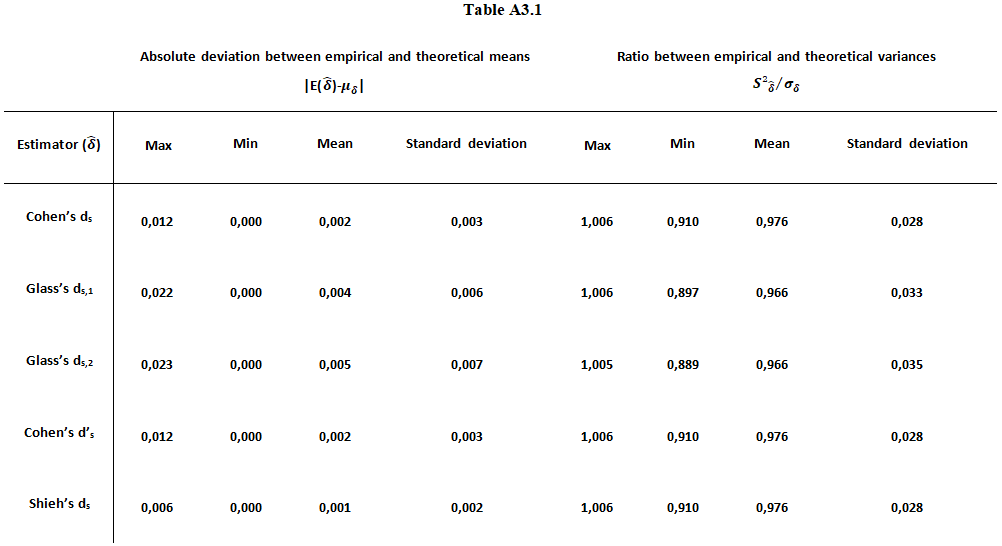
\includegraphics{D:/Documents/Github_projects/Effect-sizes/Supplemental Material 3/Files/Png tables/Table A3.1} 

}

\end{sidewaysfigure}

\begin{sidewaysfigure}

{\centering 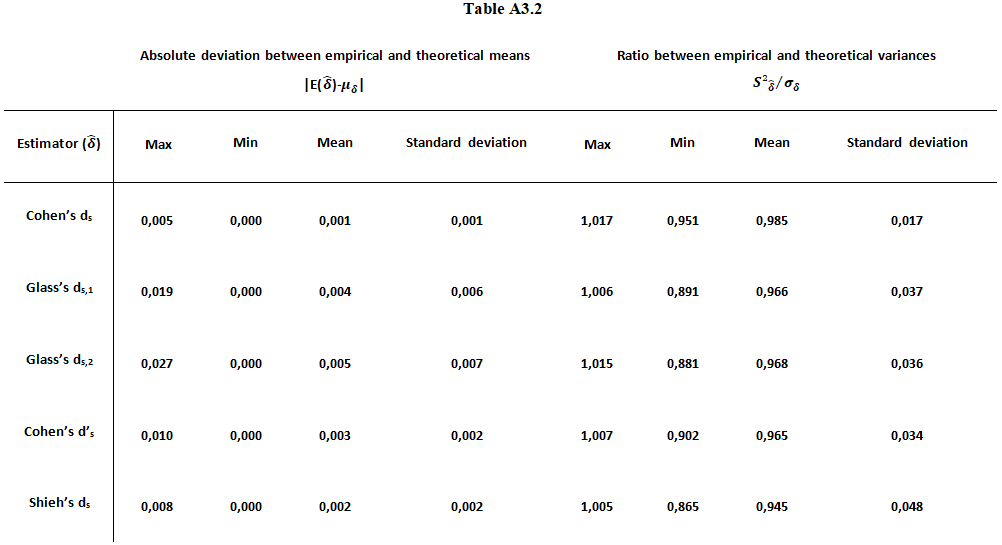
\includegraphics{D:/Documents/Github_projects/Effect-sizes/Supplemental Material 3/Files/Png tables/Table A3.2} 

}

\end{sidewaysfigure}

\begin{sidewaysfigure}

{\centering 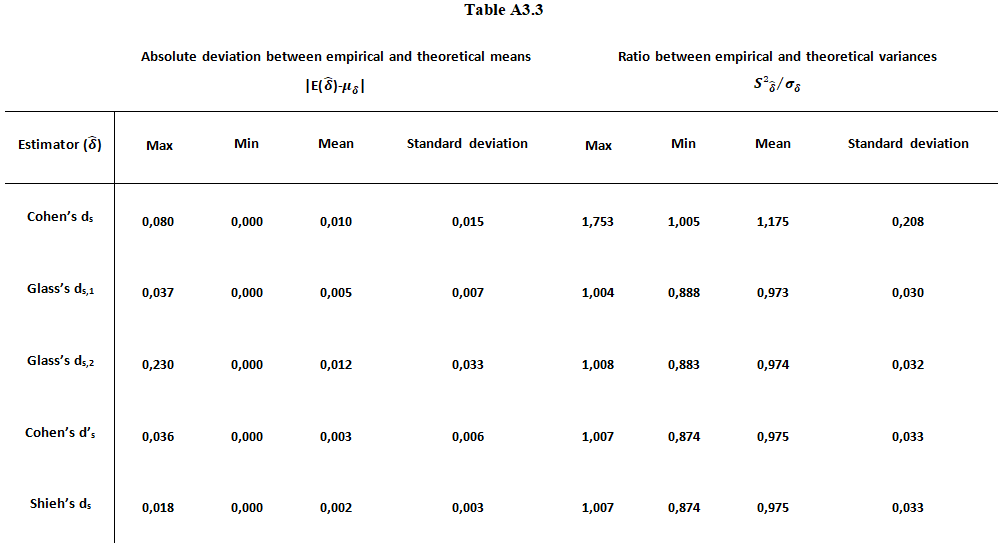
\includegraphics{D:/Documents/Github_projects/Effect-sizes/Supplemental Material 3/Files/Png tables/Table A3.3} 

}

\end{sidewaysfigure}

\begin{sidewaysfigure}

{\centering 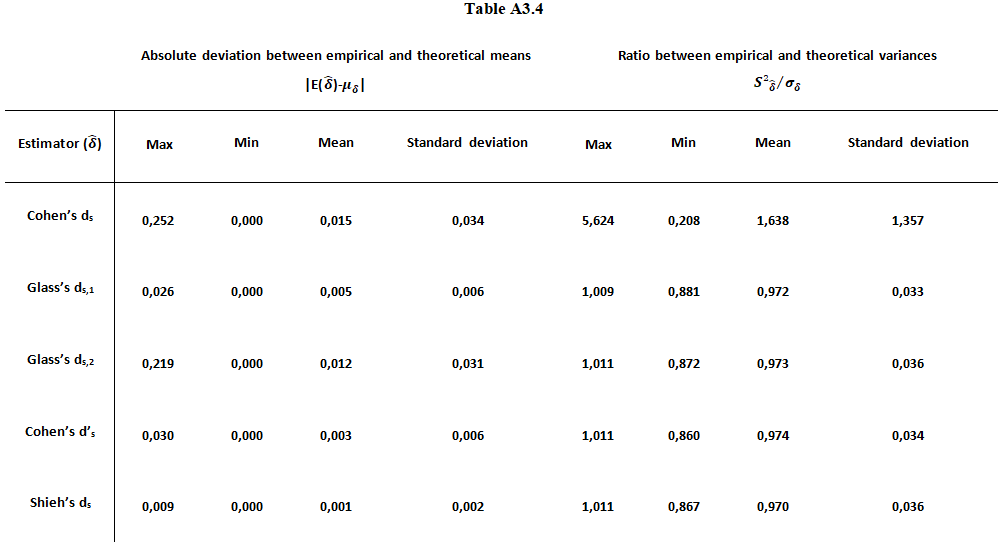
\includegraphics{D:/Documents/Github_projects/Effect-sizes/Supplemental Material 3/Files/Png tables/Table A3.4} 

}

\end{sidewaysfigure}

\begin{sidewaysfigure}

{\centering 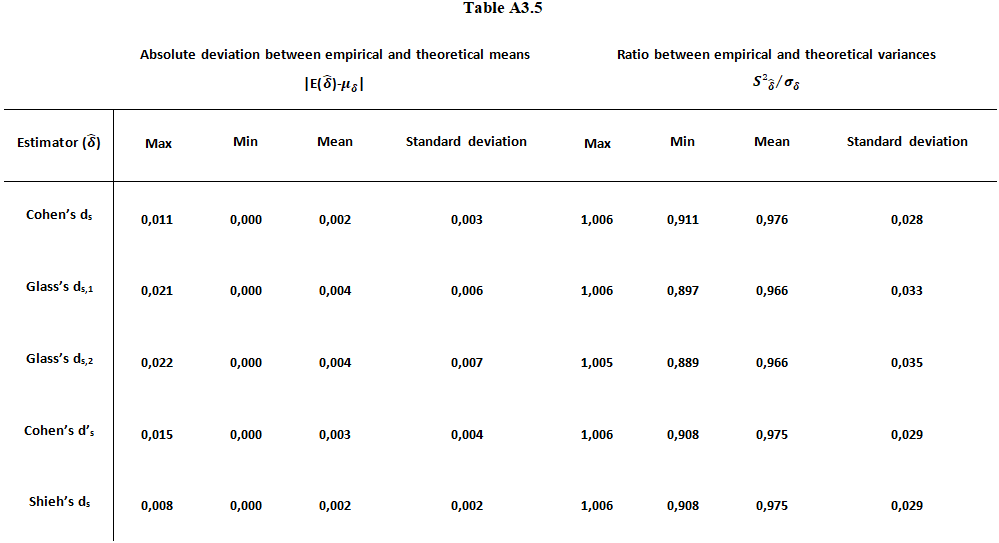
\includegraphics{D:/Documents/Github_projects/Effect-sizes/Supplemental Material 3/Files/Png tables/Table A3.5} 

}

\end{sidewaysfigure}

\begin{sidewaysfigure}

{\centering 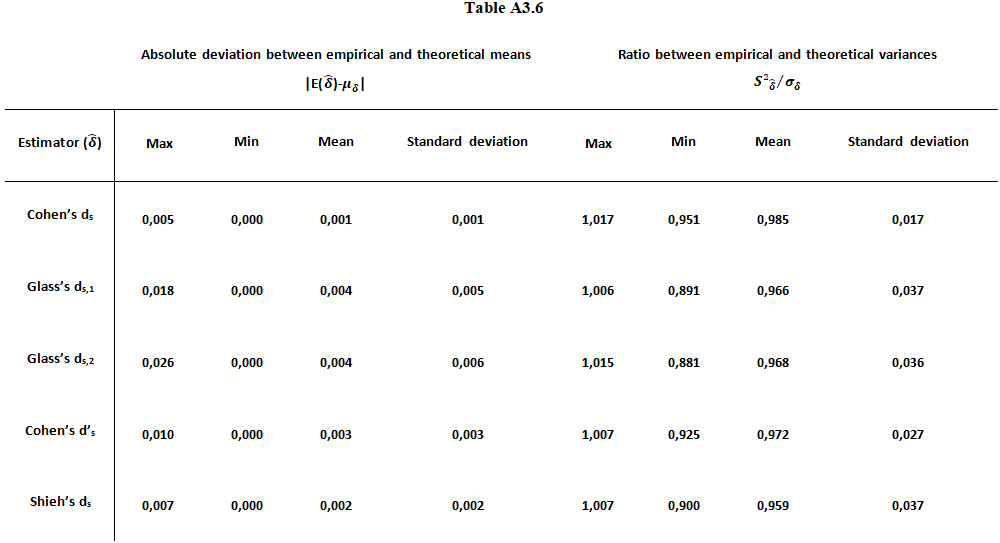
\includegraphics{D:/Documents/Github_projects/Effect-sizes/Supplemental Material 3/Files/Png tables/Table A3.6} 

}

\end{sidewaysfigure}

\begin{sidewaysfigure}

{\centering 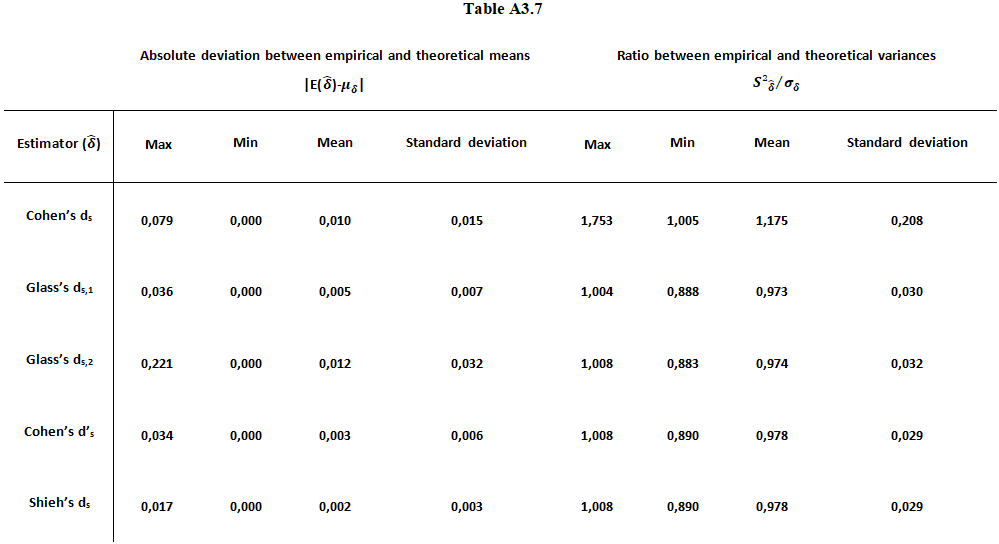
\includegraphics{D:/Documents/Github_projects/Effect-sizes/Supplemental Material 3/Files/Png tables/Table A3.7} 

}

\end{sidewaysfigure}

\begin{sidewaysfigure}

{\centering 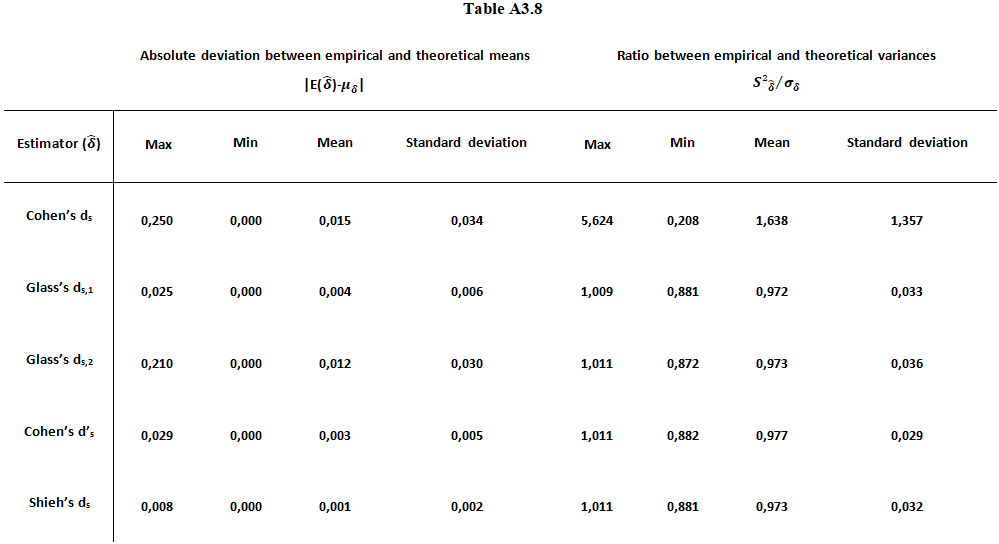
\includegraphics{D:/Documents/Github_projects/Effect-sizes/Supplemental Material 3/Files/Png tables/Table A3.8} 

}

\end{sidewaysfigure}

\end{document}
